\chapter{Background \& Objectives}

% This section should discuss your preparation for the project, including background reading, your analysis of the problem and the process or method you have followed to help structure your work.  It is likely that you will reuse part of your outline project specification, but at this point in the project you should have more to talk about. 
% 
% \textbf{Note}: 
% 
% \begin{itemize}
%    \item All of the sections and text in this example are for illustration purposes. The main Chapters are a good starting point, but the content and actual sections that you include are likely to be different.
%    
%    \item Look at the document on the Structure of the Final Report for additional guidance. 
%    
% \end{itemize}

\section{Background}
As part of the BEACON Wales\cite{beacon} project, researchers at Aberystwyth University have been studying three species of yeast, \textit{Candida tropicalis}, \textit{Candida boidinii}, and \textit{Candida shehatae}. To study the genetics of these species, they have each undergone Illumina sequencing producing a library of short reads between 80 and 120 bp in length. Each library of reads for each species was then assembled into contigs (contiguous DNA fragments). This process produces an approximate representation of the underlying species DNA, which then can then be compared to other better understood genome databases and annotated accordingly.

Arabinose and xylose are five carbon sugars ubiquitously found in plants such as grass, which can be used as a feedstock for industrial biotechnology. \textit{C. tropicalis} is able to convert arabinose and xylose into arabitol and xylitol respectively. Xylitol is a commercially valuable anti-bacterial food grade sugar use in the manufacture of chewing gum \cite{xylitol}. However arabitol and xylitol are stereo isomers and cannot be easily separated. Unlike \textit{C. tropicalis} and \textit{C. shehatae},  \textit{C. boidinii} is unable to utilise arabinose (for an unknown reason), but does process xylose into xylitol, just at a commercially unviable rate. 

Understanding at a genomic level why \textit{C. boidinii} is unable to utilise arabinose and genetically modifying \textit{C. tropicalis} to have the same phenotype, may enable \textit{C. tropicalis} to exclusively produce xylitol and not arabitol. This would provide a cost effective way to produce a source of xylitol, which can be used for many applications. One exciting possibility is using it as a low glycaemic index table sugar that can be used by those suffering from diabetes.

As Sboner et al. highlight in their paper "The real cost of sequencing: higher than you think!"\cite{sequencingcost} the cost of sequencing DNA is falling faster than Moore's law, which is in turn increasing the amount of data being produced from sequencing. The real cost of sequencing DNA is now in processing the sequence data into meaningful results, that can be studied in a wet lab experiment. 

Currently researchers have the genetic information for the three species of yeast in the form of a FASTA file containing thousands of contigs. These files are large \textgreater 16MB text files, making it difficult to extract meaningful information quickly. To make predictions about which genes encode which proteins in yeasts they will need to be able to search and browse this data in a much more accessible form.

This is why a website representing this data, and offering search functionality would be advantageous to them, as it would provide a simple and familiar user experience to other web based genome browsers such as the Candida Genome Database\cite{cgd}, which they are already familiar with and regularly use as a reference. 

\subsection{Existing Databases}
As the core of the project focuses on having the data stored in a database, the first action was to investigate the current database solutions that had been developed for genomic information. 

The most well established database is CHADO\cite{chado}, which was initially developed back in 2005 for the FlyBase\cite{flybase} project. It has since then grown to accommodate information about other model organisms such as plants, and other complex multicellular animals. It uses PostgreSQL\cite{postgres} to store it's data and Perl\cite{perl} to setup and maintain the database. Due to it's monolithic approach of being a one size fits all solution, it has over 200 tables in a very complex schema. This makes working on it rather difficult, as there are many relations to consider when entering and manipulating data from the database.

When installing and populating CHADO, it was clear that the project wasn't very well maintained as during the installation several of the Perl modules that it depends on were not able to successfully build, due to bugs in the modules causing the tests that ensure the build was made correctly to fail, and thus not install. This meant several modules had to be manually fixed just to get the application to install correctly. Additional complexity of the systems architecture stemming from it being an older project and not having the active surrounding ecosystem that other platforms may have, increases the time taken to develop for and maintain the database.

This combined with the fact that Perl now has less market share\cite{perl-market} due to the emergence of Python\cite{python} and JavaScript\cite{node} among other scripting languages, has resulted in fewer online resources available for Perl developers when compared to newer scripting languages. This is mainly due to newer languages having more popular package management, ecosystems and syntax. 

Developing the application in Perl to work with these existing platforms, would be a viable option, but this project is also an opportunity to show that genomic data can be adequately handled by newer technologies such as JavaScript and NoSQL databases.

\subsection{Alignment Tools}
The data provided by the client in this project was insufficiently documented and so it was deemed prudent to investigate how the existing data was produced. This would ensure that any new data added throughout the project was interoperable, and could be easily produced.

The original alignment tool BLAST\cite{blast} was developed in the 90's and is very widely accepted as the {\it de-facto} standard for performing alignments. 

Alignment is when a DNA, or protein sequence is compared against a database of known protein sequences that have already been determined via previous research. This allows a researcher to match their sequences against known genes and annotate them accordingly. These annotations aren't proof that genes with similar sequences have the same function, but it is a good starting point. To prove it the researchers will test it in a lab experiment, however as there are many thousands of potential genes to test it is a lot more efficient to infer function via sequence similarity before undergoing wet lab experiments.

Aligning two sequences of DNA is a computationally intensive task, that there have been many efforts to improve the efficiency of. One area that has been pursued is the use of GPU's to perform alignments in parallel, utilising hundreds or thousands of cores of the GPU, compared to the tens of cores available on modern CPU's. 

Initially Diamond\cite{diamond}, a CPU only tool, was tested and was able to align the data sets against the NCBI\cite{ncbi} non-redundant protein database\cite{nr} using the blastx algorithm to align the nucleotide sequences against the known proteins. This took about an hour and a quarter for each species, this was only using the CPU and may have been bottle necked by the mechanical drives being used for storage. It is important to note the hardware being used for this, as the time taken is determined by the hardware. The following hardware was used, Intel i7-6700k @ 4.6Ghz, 16GB of RAM, a 7200rpm Hard Disk Drive, and a Nvidia GTX 980. 

As there was a high performance graphics card available it would be advantageous to make use of a GPU accelerated alignment tool to make the most of the hardware available, and reduce the time that any future alignments may take. 

The first attempt to use a GPU powered tool was BarraCUDA\cite{barracuda}, which installed successfully and appeared to run fine, however it would attempt to read in the entire reference database into memory. This was an issue as the NCBI non-redundant database is around 66GB in size, and the system that was being used only had 16GB of RAM available. 

The next tool tested was CLAST\cite{clast}, which unfortunately had compilation errors on the system. Debugging this was out of scope for my project as in this initial stage it didn't seem necessary. Next tested was Cudasw++\cite{cudasw} this did install, but ran into the same issues as BarraCUDA, being limited by the system memory available. 

In an attempt to get GPU acceleration working, the NCBI nr database was split up into 10GB chunks for use with these tools, however even after being reduced in size, BarraCUDA and Cudasw++ both had errors and failed to complete an alignment. 

It was decided that although the speed gains of a GPU accelerated alignment tool would be significant, the Diamond alignment was quick enough to not be a major bottleneck for the project, when compared with the extra time and effort that would have to be put into investigating how to get the GPU alignments to work. 

\section{Analysis}
% Taking into account the problem and what you learned from the background work, what was your analysis of the problem? 

From researching the current solutions to the problem of annotating, storing and presenting genetic information, it was clear that a complete solution using modern web development technologies such as Node.js wasn't currently in the public or open source domain. 

Of the open source projects that were currently in use the majority appeared to be very old and monolithic. This is often due to their integration with the most popular genome viewers GBrowse\cite{gbrowse} and JBrowse\cite{jbrowse} which are both written in Perl.

Perl is less suited to modern web development than some of the newer languages, mainly due to it's smaller market share\cite{perl-market} and greatly smaller number of available third party modules, and support.

\begin{figure}[ht!]
\begin{center}
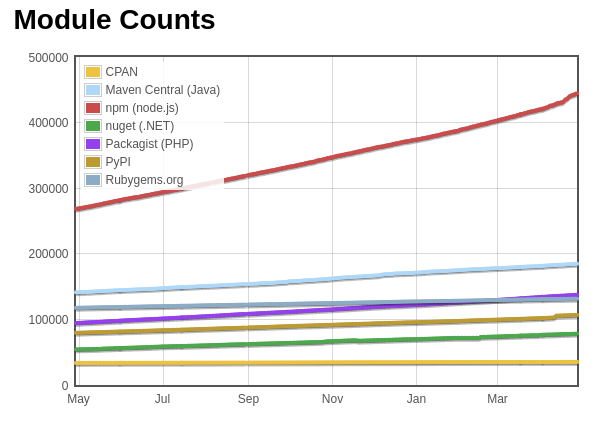
\includegraphics[scale=0.7]{module-count}
\caption{Number of modules available for server side languages, Perl (CPAN), Java (Maven), JavaScript (npm), .NET (nuget), PHP (Packagist), Python (PyPI), Ruby (Gems)\cite{modulecounts}}
\end{center}
\end{figure}

Web development in Perl is clearly on the decline as seen by it's market share\cite{perl-market}, and that means that the ecosystem surrounding it just can't compete with newer technologies such as Ruby on Rails or Node.js.

\subsection{Analysis of the problem}
Looking at the data that I was provided with there was three clear stages to the development of my solution. The first would be to ensure that the data I had was valid and in the same format for each of the species that were being analysed. The next was to import that data into a database, and then from there develop a web front end to interact with the data in the database. 

An alternative approach to this project would be to use one of the existing databases such as Intermine\cite{intermine} or CHADO\cite{chado}, and then use a web front end compatible with those databases such as GBrowse\cite{gbrowse} or JBrowse\cite{jbrowse}. This would require changes to how the data was processed before going into these established systems, however the benefit of using this approach would be access to all of the bioinformatics tools that are compatible with these platforms.

As a computer scientist looking at this problem, there doesn't seem to be much need for a very complex solution. Once the data is generated, it just needs to be made into a database friendly format and then stored in a database. From there building a simple web front end to make the database accessible is a simple task. There isn't any need to manipulate or modify the data, simply create and read it. As the requirements for the system were so simple, one of the more advanced projects like CHADO and GBrowse, didn't seem necessary, as although mature and well supported in Bioinformatics they come with a lot of extra features that wouldn't be required and just add bloat to the project. 

  \subsection{Comparison of SQL and NoSQL databases}
  Structured Query Language (SQL) databases such as MariaDB, PostrgeSQL and SQLite, store data in a relational manner, this means that data is stored across many linked tables, that are grouped by the data type. They are the interfaced with via SQL to select related data from multiple tables to return a meaningful result. 
  
  \begin{itemize}
    \item SQL based systems have been used for a long time and have a large amount of support and compatibility with different frameworks. 
    \item Efficient storage of data, as data is put into first normal form and not replicated.
    \item Complex queries can be ran with relative ease.
    \item Requires a strict schema.
    \item Development is more complex as you have to manage and maintain relations.
  \end{itemize}

  NoSQL databases store data in collections of documents. Each collection is usually linked to a use case for the data, for example a website that has blog posts would have a `blog' collection, that stores all of the data for blog posts. The collection is made up of individual documents representing individual items, so the `blog' collection will store lots of individual blog posts. Each document is then made up of key value pairs, commonly represented as JSON.\@

  \begin{itemize}
    \item Collections are based on use cases so no complex selection logic.
    \item Data is represented as JSON so it is very interoperable with JavaScript.
    \item Dynamic schema, not every document has to have the same information as the other documents in the collection.
    \item Newer technology so less legacy support.
    \item Data can be stored twice which is a less efficient use of disk space.
  \end{itemize}

The decision on which technology to use is discussed in the Design section. 

\section{Research Method and Software Process}
It was intended to use a blend of agile and extreme programming methodologies for this project. The idea was to ensure that as the understanding of the task at hand increased and new requirements or changes to the structure of the application became necessary, an agile workflow would allow adaptations to be made without setting the project's progress back. 


For this project there were clearly defined clients that could be accessed and used for feedback during development iterations. David Bryant and Abhishek Somani, the scientists conducting the research, were available for meetings to provide feed back and discuss progress of the project. 

When suitable we would meet on a Friday at the end of an iteration to discuss the projects progress and any difficulties that may have been encountered. Towards the end of the project this time was used to get detailed feedback on how the website could be improved. 
Unit testing was also used to develop the key algorithms, as well as continuous integration and deployment, this process is described in much more detail later on in the document. It was key to being able to deliver working software at regular intervals and demonstrate it to the clients. 

Once requirements were gathered a Kanban board would be made with each individual task listed, based on the requirements of the application. Those tasks would then be weighted with an estimated difficulty, and then worked on. Once development had started on each task it would be moved to the "In progress" board, and then across to the "Done" board, once completed. 

\begin{figure}[ht!]
\begin{center}
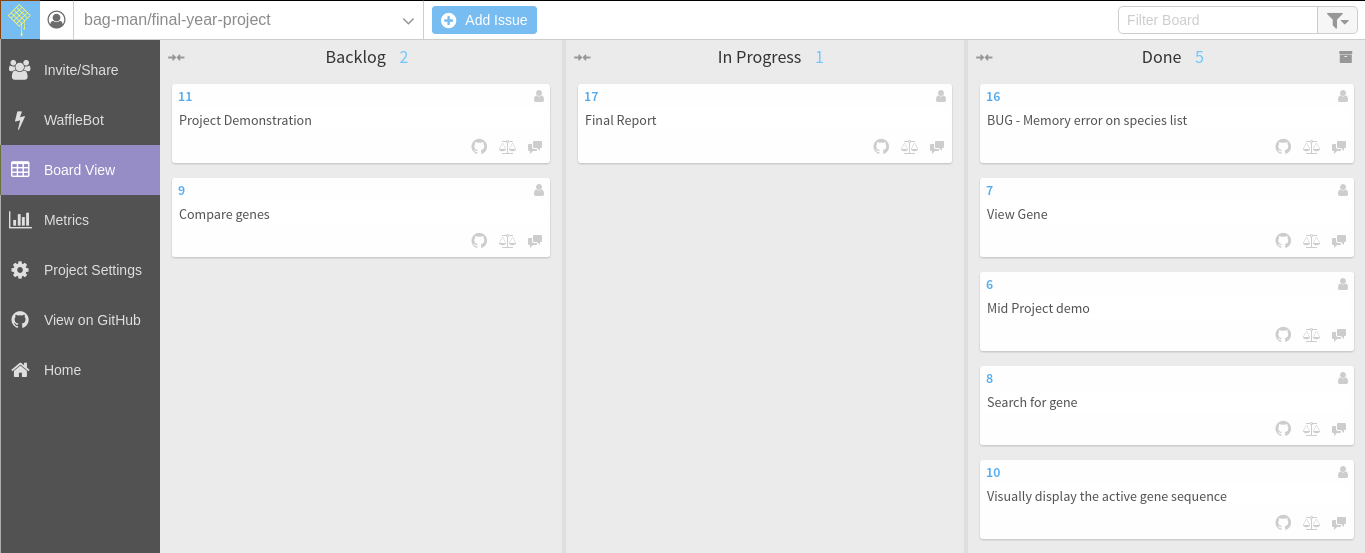
\includegraphics[scale=0.3]{waffle}
\caption{Kanban board in use. Waffle.io is the service providing the board}
\end{center}
\end{figure}

However as this project involved a lot of domain knowledge that wasn't familiar, there was a very significant amount of time spent learning what the data meant and how it should be used. During that time I was prototyping potential solutions to how the data could be interpreted, without a specific set of requirements in mind. This lead to very vague requirements being created and development following a path closely linked to the data and the understanding of it. 

An example of this process was the reverse compliment feature, that didn't appear to be necessary until a couple of weeks before the project deadline. This is exactly why a traditional structured development process like waterfall would not have worked for this project, as new requirements and features were appearing deep into the project, something that wouldn't have been able to be accommodated for if using a strict waterfall model, where each phase of development is scheduled a head of time.

% You need to describe briefly the life cycle model or research method that you used. You do not need to write about all of the different process models that you are aware of. Focus on the process model or research method that you have used. It is possible that you needed to adapt an existing method to suit your project; clearly identify what you used and how you adapted it for your needs.

% For the research-oriented projects, there needs to be a suitable process for the construction of the software elements that support your work. 
